% P08-F03 universal preprocessing renderer output -- copied estimates only
%% source SHA256: 8c910290a3d09cbc9f03e7dcde77ae1598487533b0c68cfa1709a42e7d38621d
%% semantic SHA256: 7045e1dc2788300144330414456a5725a0e4cd3af23681b05b2c9e546cf3b73c
\documentclass[border=0pt]{standalone}
\usepackage[T1]{fontenc}
\usepackage[utf8]{inputenc}
\usepackage{lmodern}
\usepackage{tikz}
\usepackage{pgfplots}
\pgfplotsset{compat=1.18}
\definecolor{PolA}{HTML}{0072B2}
\pgfplotsset{pt0/.style={only marks, mark=*, color=PolA, mark options={fill=PolA, draw=black}}}
\pgfplotsset{bar0/.style={PolA, line width=0.8pt, mark=|, mark options={color=PolA}}}
\definecolor{PolB}{HTML}{D55E00}
\pgfplotsset{pt1/.style={only marks, mark=square*, color=PolB, mark options={fill=PolB, draw=black}}}
\pgfplotsset{bar1/.style={PolB, line width=0.8pt, mark=|, mark options={color=PolB}}}
\pgfplotsset{domainpts/.style={only marks, mark=o, mark options={draw=gray, fill=none, scale=0.7}}}
\tikzset{intervalna/.style={font=\fontsize{8}{10}\selectfont, anchor=east}}
\begin{document}
\begin{minipage}{181.86mm}\centering
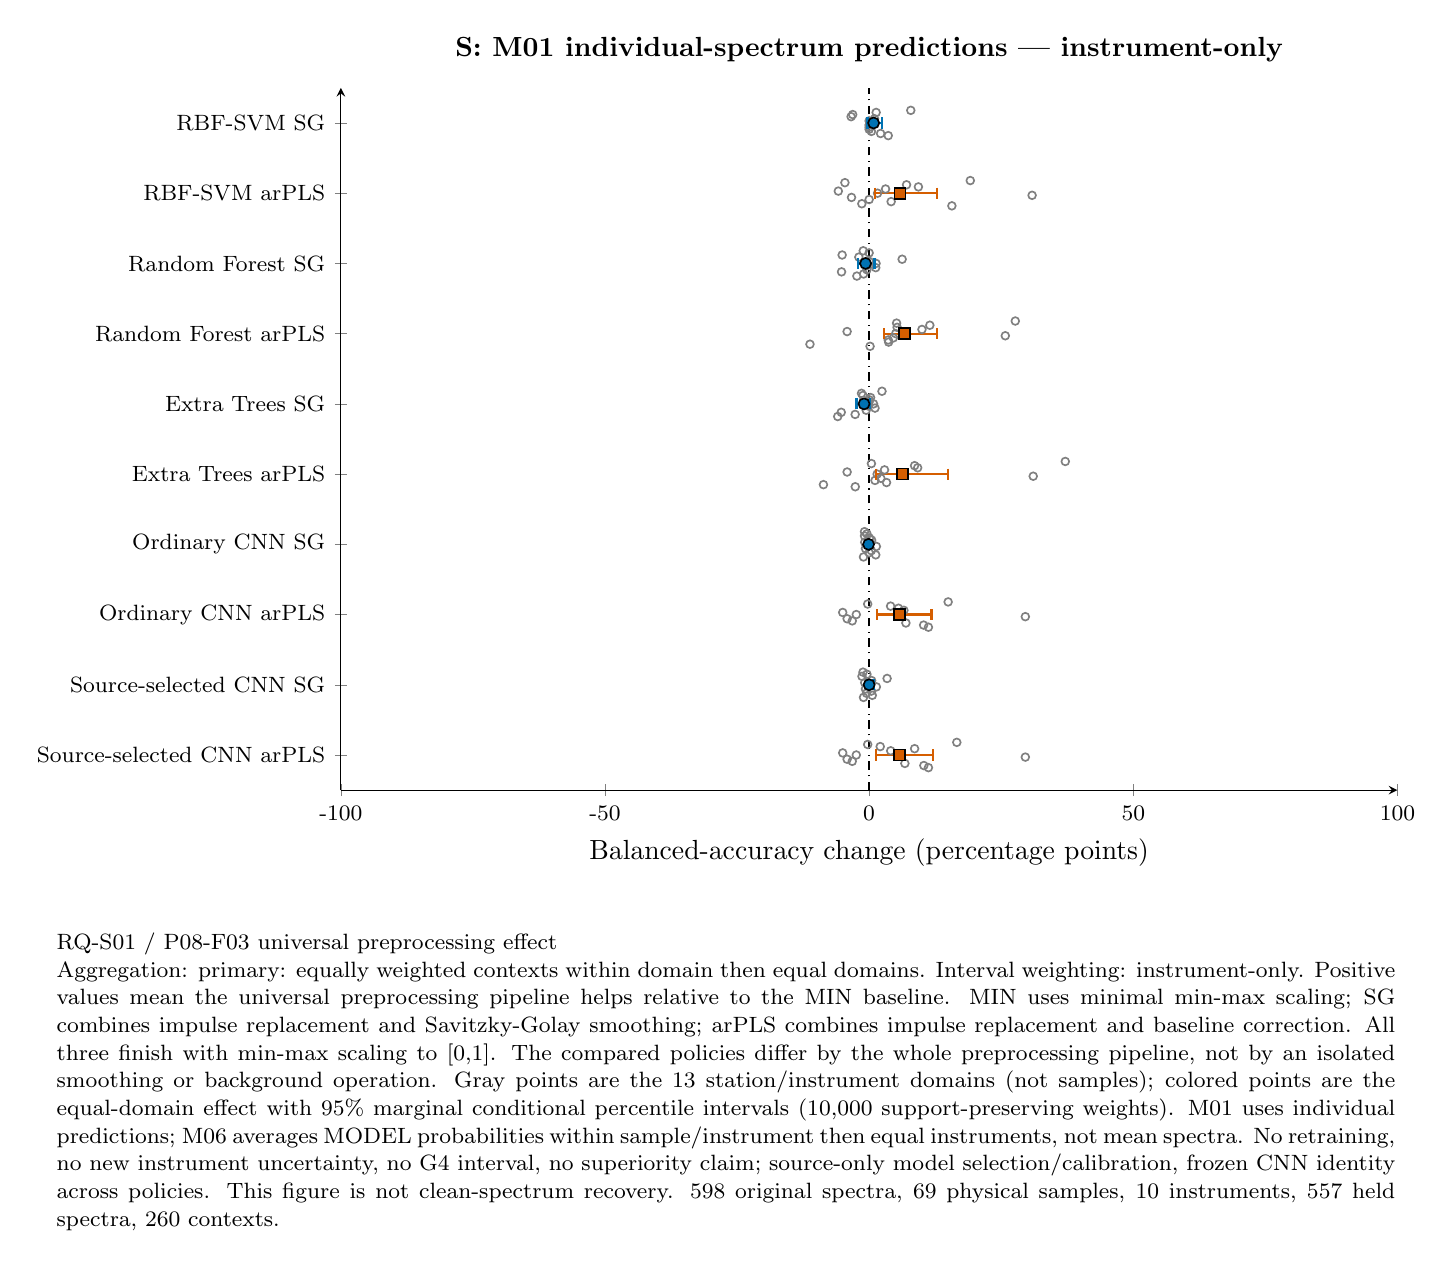
\begin{tikzpicture}
\begin{axis}[width=150mm, height=105mm, clip=false, xmin=-1, xmax=1, xtick={-1,-0.5,0,0.5,1}, xticklabels={-100,-50,0,50,100}, xlabel={Balanced-accuracy change (percentage points)}, ymin=-0.5, ymax=9.5, ytick={0,1,2,3,4,5,6,7,8,9}, yticklabels={{Source-selected CNN arPLS}, {Source-selected CNN SG}, {Ordinary CNN arPLS}, {Ordinary CNN SG}, {Extra Trees arPLS}, {Extra Trees SG}, {Random Forest arPLS}, {Random Forest SG}, {RBF-SVM arPLS}, {RBF-SVM SG}}, yticklabel style={font=\fontsize{8}{10}\selectfont}, tick label style={font=\fontsize{8}{10}\selectfont}, axis lines=left, title={S: M01 individual-spectrum predictions | instrument-only}, title style={font=\bfseries\fontsize{10}{12}\selectfont}, every axis plot/.append style={line width=0.6pt}]
\draw[black, dash dot, line width=0.6pt] (axis cs:0,-0.5) -- (axis cs:0,9.5);
\addplot[domainpts] coordinates {(0.03616462241462242,8.8200000000000003) (0.021719576719576719,8.8499999999999996) (0.0042857142857142833,8.8800000000000008) (0,8.9100000000000001) (0,8.9399999999999995) (0,8.9700000000000006) (0.011111111111111106,9) (0,9.0299999999999994) (0.010277777777777778,9.0600000000000005) (-0.034126984126984124,9.0899999999999999) (-0.03111111111111111,9.1199999999999992) (0.013293650793650792,9.1500000000000004) (0.0788498075998076,9.1799999999999997)};
\addplot[bar0] coordinates {(-0.0030410281642613154,9) (0.024759352655302248,9)};
\addplot[pt0] coordinates {(0.0084972434972434962,9)};
\addplot[domainpts] coordinates {(0.1566480278980279,7.8200000000000003) (-0.013809523809523817,7.8499999999999996) (0.041666666666666664,7.8799999999999999) (0,7.9100000000000001) (-0.033333333333333326,7.9400000000000004) (0.30849867724867719,7.9699999999999998) (0.015972222222222221,8) (-0.058333333333333327,8.0299999999999994) (0.031111111111111117,8.0600000000000005) (0.093293650793650804,8.0899999999999999) (0.070833333333333331,8.1199999999999992) (-0.045833333333333337,8.1500000000000004) (0.19146464646464648,8.1799999999999997)};
\addplot[bar1] coordinates {(0.010562993578955914,8) (0.12911279920053084,8)};
\addplot[pt1] coordinates {(0.058321447071447069,8)};
\addplot[domainpts] coordinates {(-0.02322811447811448,6.8200000000000003) (-0.010449735449735452,6.8499999999999996) (-0.052222222222222239,6.8799999999999999) (-0.0041666666666666666,6.9100000000000001) (0.012500000000000001,6.9400000000000004) (-0.0039351851851851848,6.9699999999999998) (0.013055555555555553,7) (0,7.0300000000000002) (0.0625,7.0599999999999996) (-0.019444444444444445,7.0899999999999999) (-0.051071428571428559,7.1200000000000001) (0,7.1500000000000004) (-0.011138768638768637,7.1799999999999997)};
\addplot[bar0] coordinates {(-0.021593486900971525,7) (0.010234979347029898,7)};
\addplot[pt0] coordinates {(-0.0067385392385392396,7)};
\addplot[domainpts] coordinates {(0.0017646705146705185,5.8200000000000003) (-0.11198412698412696,5.8499999999999996) (0.036944444444444446,5.8799999999999999) (0.036111111111111108,5.9100000000000001) (0.045833333333333337,5.9400000000000004) (0.25774801587301593,5.9699999999999998) (0.050277777777777775,6) (-0.041666666666666664,6.0300000000000002) (0.10000000000000001,6.0599999999999996) (0.052976190476190468,6.0899999999999999) (0.11492063492063494,6.1200000000000001) (0.051944444444444446,6.1500000000000004) (0.27665644540644541,6.1799999999999997)};
\addplot[bar1] coordinates {(0.02838956107991146,6) (0.12899812700261648,6)};
\addplot[pt1] coordinates {(0.067040482665482667,6)};
\addplot[domainpts] coordinates {(-0.059430615680615681,4.8200000000000003) (-0.026455026455026454,4.8499999999999996) (-0.052777777777777771,4.8799999999999999) (-0.0055555555555555549,4.9100000000000001) (0.01111111111111111,4.9400000000000004) (-0.0016666666666666666,4.9699999999999998) (0.0083333333333333332,5) (0,5.0300000000000002) (0,5.0599999999999996) (0.0027777777777777792,5.0899999999999999) (-0.011785714285714285,5.1200000000000001) (-0.014444444444444444,5.1500000000000004) (0.024325396825396826,5.1799999999999997)};
\addplot[bar0] coordinates {(-0.023845107354877309,5) (0.0012852653484898612,5)};
\addplot[pt0] coordinates {(-0.0096590909090909071,5)};
\addplot[domainpts] coordinates {(-0.026245189995189995,3.8199999999999998) (-0.086481481481481493,3.8500000000000001) (0.032936507936507937,3.8799999999999999) (0.01111111111111111,3.9100000000000001) (0.02222222222222222,3.9399999999999999) (0.31058531746031737,3.9700000000000002) (0.015138888888888886,4) (-0.041666666666666664,4.0300000000000002) (0.029166666666666667,4.0599999999999996) (0.091865079365079372,4.0899999999999999) (0.086031746031746043,4.1200000000000001) (0.0043055555555555564,4.1500000000000004) (0.3712999037999038,4.1799999999999997)};
\addplot[bar1] coordinates {(0.013579643599790353,4) (0.14941826705253727,4)};
\addplot[pt1] coordinates {(0.063097666222666215,4)};
\addplot[domainpts] coordinates {(-0.010674603174603173,2.8199999999999998) (0.012539682539682536,2.8500000000000001) (6.9388939039072288e-19,2.8799999999999999) (0.0041666666666666657,2.9100000000000001) (-0.0069444444444444423,2.9399999999999999) (0.013683862433862434,2.9700000000000002) (-0.0025000000000000001,3) (-0.0083333333333333332,3.0299999999999998) (0.0047222222222222214,3.0600000000000001) (0.0006944444444444448,3.0899999999999999) (-0.0087301587301587304,3.1200000000000001) (-0.0041666666666666657,3.1499999999999999) (-0.0087632275132275145,3.1800000000000002)};
\addplot[bar0] coordinates {(-0.0043547378144874922,3) (0.0026343103951175693,3)};
\addplot[pt0] coordinates {(-0.0011004273504273505,3)};
\addplot[domainpts] coordinates {(0.11224025974025971,1.8200000000000001) (0.10314814814814814,1.8500000000000001) (0.069603174603174583,1.8799999999999999) (-0.031944444444444442,1.9099999999999999) (-0.041666666666666671,1.9399999999999999) (0.29567791005291,1.97) (-0.024325396825396826,2) (-0.050000000000000003,2.0299999999999998) (0.065833333333333327,2.0600000000000001) (0.055555555555555546,2.0899999999999999) (0.040634920634920628,2.1200000000000001) (-0.0027380952380952387,2.1499999999999999) (0.14956709956709954,2.1800000000000002)};
\addplot[bar1] coordinates {(0.014804135447326006,2) (0.11802193930963784,2)};
\addplot[pt1] coordinates {(0.05704506142006141,2)};
\addplot[domainpts] coordinates {(-0.010674603174603173,0.82000000000000006) (0.0059920634920634904,0.84999999999999998) (-0.005000000000000001,0.88) (0.0041666666666666657,0.91000000000000003) (-0.0069444444444444423,0.93999999999999995) (0.013683862433862434,0.96999999999999997) (-0.0025000000000000001,1) (-0.0083333333333333332,1.03) (0.0047222222222222214,1.0600000000000001) (0.034027777777777782,1.0900000000000001) (-0.013492063492063491,1.1200000000000001) (-0.0041666666666666657,1.1499999999999999) (-0.011607142857142861,1.1799999999999999)};
\addplot[bar0] coordinates {(-0.0047360694744332668,1) (0.0081439507589989683,1)};
\addplot[pt0] coordinates {(-9.666259666259603e-06,1)};
\addplot[domainpts] coordinates {(0.11224025974025971,-0.17999999999999999) (0.10354497354497354,-0.14999999999999999) (0.067658730158730154,-0.12) (-0.031944444444444442,-0.089999999999999997) (-0.041666666666666671,-0.059999999999999998) (0.29567791005291,-0.029999999999999999) (-0.024325396825396826,0) (-0.050000000000000003,0.029999999999999999) (0.040833333333333333,0.059999999999999998) (0.086111111111111097,0.089999999999999997) (0.020992063492063492,0.12) (-0.0027380952380952387,0.14999999999999999) (0.16595598845598844,0.17999999999999999)};
\addplot[bar1] coordinates {(0.013618012730222088,0) (0.12031940808836267,0)};
\addplot[pt1] coordinates {(0.057103058978058965,0)};
\end{axis}
\node[anchor=north, align=justify, text width=170mm, font=\fontsize{8}{10}\selectfont] at ([yshift=-6mm]current bounding box.south) {RQ-S01 / P08-F03 universal preprocessing effect\\ Aggregation: primary: equally weighted contexts within domain then equal domains. Interval weighting: instrument-only. Positive values mean the universal preprocessing pipeline helps relative to the MIN baseline. MIN uses minimal min-max scaling; SG combines impulse replacement and Savitzky-Golay smoothing; arPLS combines impulse replacement and baseline correction. All three finish with min-max scaling to [0,1]. The compared policies differ by the whole preprocessing pipeline, not by an isolated smoothing or background operation. Gray points are the 13 station/instrument domains (not samples); colored points are the equal-domain effect with 95\% marginal conditional percentile intervals (10,000 support-preserving weights). M01 uses individual predictions; M06 averages MODEL probabilities within sample/instrument then equal instruments, not mean spectra. No retraining, no new instrument uncertainty, no G4 interval, no superiority claim; source-only model selection/calibration, frozen CNN identity across policies. This figure is not clean-spectrum recovery. 598 original spectra, 69 physical samples, 10 instruments, 557 held spectra, 260 contexts.};
\end{tikzpicture}
\end{minipage}
\end{document}
